
% Comandos de dados - titulo do documento
\newcommand{\titulo}[1]{\title{#1}}
\newcommand{\imprimirtitulo}{\thetitle}

% Comandos de dados - autor (use \and para múltiplos autores)
\newcommand{\autor}[1]{\author{#1}}
\newcommand{\imprimirautor}{\theauthor}

% Comandos de dados - data
\let\olddate\date
\renewcommand{\date}[1]{\AtBeginDocument{\olddate{#1}}}
\newcommand{\data}[1]{\date{#1}}
\newcommand{\imprimirdata}{
  \center
  \the\year
}

% Comandos de dados - instituição
\providecommand{\imprimirinstituicao}{}
\newcommand{\instituicao}[1]{\renewcommand{\imprimirinstituicao}{#1}}

% Comandos de dados - local
\providecommand{\imprimirlocal}{}
\newcommand{\local}[1]{\renewcommand{\imprimirlocal}{#1}}

% Comandos de dados - preambulo
\providecommand{\imprimirpreambulo}{}
\newcommand{\preambulo}[1]{\renewcommand{\imprimirpreambulo}{#1}}

% Comandos de dados - orientador
\providecommand{\imprimirorientadorRotulo}{}
\providecommand{\imprimirorientador}{}
\newcommand{\orientador}[2][\orientadorname]%
  {\renewcommand{\imprimirorientadorRotulo}{#1}%
   \renewcommand{\imprimirorientador}{#2}}

% Comandos de dados - coorientador
\providecommand{\imprimircoorientadorRotulo}{}
\providecommand{\imprimircoorientador}{}
\newcommand{\coorientador}[2][\coorientadorname]%
  {\renewcommand{\imprimircoorientadorRotulo}{#1}%
   \renewcommand{\imprimircoorientador}{#2}}

% Comandos de dados - tipo de trabalho
\providecommand{\imprimirtipotrabalho}{}
\newcommand{\tipotrabalho}[1]{\renewcommand{\imprimirtipotrabalho}{#1}}


\newcommand{\imprimircapa}{%
  \begin{capa}%
    \center
    \imprimirinstituicao
    \vfill
    \large\imprimirautor

    \vfill
    \begin{center}
      \MakeUppercase{\imprimirtitulo}
    \end{center}
    \vfill

    \large\imprimirlocal

    \large\imprimirdata

    \vspace*{1cm}
  \end{capa}
}

\newenvironment{capa}{\begin{titlingpage}}{\end{titlingpage}\cleardoublepage}

% ---
% Folha de rosto
%   usar \imprimirfolhaderosto* caso deseje imprimir algo no verso da
%   página no caso de estar no modo twoside. Util para imprimir a Ficha
%   Bibliográfica. Porem, se estiver no modo oneside, a versao sem estrela é idêntica.
\newenvironment{folhaderosto}[1][\folhaderostoname]{\clearpage}{\cleardoublepage}
\newenvironment{folhaderosto*}[1][\folhaderostoname]{\clearpage}{\newpage}%

% ---
% Conteudo padrao da Folha de Rosto
\makeatletter
\newcommand{\folhaderostocontent}{
  \begin{center}
    \imprimirinstituicao\vspace*{\fill}

    \large\imprimirautor

    \vspace*{\fill}\vspace*{\fill}
    \begin{center}
      \MakeUppercase{\imprimirtitulo}
    \end{center}
    \vspace*{\fill}

    \hspace{.45\textwidth}
    \begin{minipage}{.5\textwidth}
       \singlespacing
       \imprimirpreambulo
     \end{minipage}
     \vspace*{\fill}

    \large\imprimirlocal
    \par
    \large\imprimirdata
    \vspace*{1cm}

  \end{center}
}
\makeatother

\newcommand{\imprimirfolhaderostostar}[1]{%
  \begin{folhaderosto*}{#1}
     \folhaderostocontent
  \end{folhaderosto*}}

\newcommand{\imprimirfolhaderostonostar}[1]{%
  \begin{folhaderosto}{#1}
     \folhaderostocontent
  \end{folhaderosto}}

\makeatletter
\newcommand{\imprimirfolhaderosto}[1][\folhaderostoname]{%
   \@ifstar
     \imprimirfolhaderostostar
     \imprimirfolhaderostonostar
}
\makeatother


\documentclass[11.5pt]{article}
\usepackage{titling}
\usepackage{sbc-template}
\usepackage{graphicx,url}
\usepackage[brazil]{babel}
\usepackage[utf8]{inputenc}

\usepackage{multicol}
\usepackage{multirow}
\usepackage{setspace,lipsum}
\usepackage[toc,page]{appendix}

\sloppy

\date{\today}

%%%%%%%%%%%%%%%%%%%%%%%%%%%%%%%%%%%%%%%%%%%%%%%%%%%%%%%%%%%%%%%%%%%%%%%%%%%%%%%%%%%%%%%%%%%%%%%%%%%%

\title{
    Estudo de Caso da Correlação Entre Cobertura de Código e Falhas Reportadas em um Sistema
    Operacional
}

\local{Porto Alegre}

\author{George Redivo Pinto}

\preambulo{Trabalho apresentado à disciplina Engenharia de Software Aplicada, pelo Curso de
Especialização em Engenharia de Software da Universidade do Vale do Rio dos Sinos - UNISINOS,
ministrada pela professora Josiane Brietzke Porto.}

\address{
  Universidade do Vale do Rio dos Sinos (UNISINOS)\\
  Porto Alegre -- RS -- Brasil
}

\instituicao{
    UNIVERSIDADE DO VALE DO RIO DOS SINOS – UNISINOS

    UNIDADE ACADÊMICA DE PESQUISA E PÓS-GRADUAÇÃO

    ESPECIALIZAÇÃO EM ENGENHARIA DE SOFTWARE
}

\begin{document}

\imprimircapa
\imprimirfolhaderosto

\maketitle

\begin{abstract}

Software testing is an important step in software development cycle. This step aims to ensure that
the code works according to the specification.
Code coverage is a metric that tries to measure the test quality by indicating the percentage of
code that were used during test execution.
This article aims to research the correlation between code coverage rate and software quality,
measured by reported faults.
To do that it was done a case study using the features of an operational system and the results
indicate that there is a correlation between code coverage rate and software quality.

\end{abstract}

\begin{resumo}

O teste de \textit{software} é uma importante etapa no processo de desenvolvimento de \textit{software}. Essa etapa
visa garantir que o \textit{software} funciona de acordo com as especificações.
A cobertura de código é uma métricas que se propõe a medir a qualidade de um teste. Ela consiste em
prover uma taxa percentual que indica a porcentagem de código executadas nos testes.
O presente artigo visa estudar se existe ou não correlação entre a cobertura de código e a
qualidade do \textit{software}, medida em quantidade de falhas reportadas.
Para tal, foi feito um estudo de caso utilizando as funcionalidades de um sistema operacional,
chegando em um resultado que indica a existência de correlação entre cobertura de ódigo e
qualidade de \textit{software}.


\end{resumo}


%%%%%%%%%%%%%%%%%%%%%%%%%%%%%%%%%%%%%%%%%%%%%%%%%%%%%%%%%%%%%%%%%%%%%%%%%%%%%%%%%%%%%%%%%%%%%%%%%%%%
%%%%%%%%%%%%%%%%%%%%%%%%%%%%%%%%%%%%%%%%%%%%%%%%%%%%%%%%%%%%%%%%%%%%%%%%%%%%%%%%%%%%%%%%%%%%%%%%%%%%
%%%%%%%%%%%%%%%%%%%%%%%%%%%%%%%%%%%%%%%%%%%%%%%%%%%%%%%%%%%%%%%%%%%%%%%%%%%%%%%%%%%%%%%%%%%%%%%%%%%%


\section{Introdução}

A etapa de teste de \textit{software} é uma etapa importante no processo de desenvolvimento de
\textit{software} e está cada vez mais presente no cotidiano das equipes de desenvolvimento de
\textit{software}.
Essa etapa visa garantir a funcionalidade de um dado \textit{software}, podendo ser feita utilizando
diversos métodos e em diversos níveis, de acordo com a finalidade do teste.
Contudo, o desenvolvimento de testes implica em um impacto financeiro no projeto, uma vez que muitas
horas e profissionais são demandados para a escrita de testes.

A cobertura de código é uma métrica que indica a porcentagem de código que está sendo coberta pelos
testes executados.
Essa métrica ajuda a medir a qualidade dos casos de teste em questão e também pode servir como uma
métrica que indica quando podemos parar de escrever testes, ou seja, quando já temos uma quantidade
suficiente de testes para cobrir um determinado código, com a finalidade de redução de custos.
Contudo, a decisão pela parada da escrita de testes pode impactar na qualidade do \textit{software}
final, uma vez que alguns casos de uso podem ficar descoberto pelos testes.
Por esse motivo é imprescindível que tal decisão seja tomada baseada em dados sólidos, a fim de
evitar esforços excessivos no desenvolvimento de teste, porém garantindo a qualidade do
\textit{software}.
Segundo \cite{coverageAtGoogle}, a adoção da análise de cobertura de código vem crescendo ao longo
dos anos e tem uma boa avaliação de seus usuários quanto à sua efetividade, o que reafirma a
necessidade de que se tenha um bom conhecimento sobre a efetividade de tal métrica para medir
qualidade de teste e de \textit{software}.

Diversos estudos tentam verificar se existe, de fato, uma correlação entre cobertura de testes e
qualidade de \textit{software}, tais como \cite{coverageMetaAnalysis}, \cite{unitTestedCrash} e
\cite{coverageLargeScaleStudy}.
Os resultados obtidos por esses estudos são controversos entre si.
\cite{coverageMetaAnalysis} traz uma revisão sistemática de diversos artigos publicados sobre o
assunto e aponta algumas possíveis vulnerabilidades metodológicas nos artigos estudados, o que
sugere que mais estudos podem ser feitos para tentar delinear melhor a relação entre cobertura de
código e qualidade de \textit{software}.

Nesse sentido, o presente artigo tem por objetivo responder a seguinte questão de pesquisa:
existe correlação entre cobertura de código e qualidade de \textit{software} de um sistema
operacional embarcado, sendo cobertura de linhas a métrica de cobertura de código e número de falhar
reportadas a métrica de qualidade de \textit{software}?
Para tal, o estudo tem o objetivo de fazer um estudo de caso, conforme descrito em
\cite{metodosPesquisa}, em um projeto de sistema operacional embarcado desenvolvido por uma empresa
brasileira, observando as métricas supracitadas e usando métodos estatísticos para identificar a
correlação entre cobertura de código e qualidade de \textit{software}.
Nesse contexto, as seguintes etapas serão desenvolvidas:

\begin{itemize}
    \item Coletar dados de cobertura de código (por repositório) e falhas reportadas do projeto (por
          funcionalidade);

    \item Sanitizar dados, excluindo dados inválidos para a pesquisa;

    \item Relacionar os repositórios com as funcionalidades;

    \item Fazer análise estatística dos dados coletados.
\end{itemize}

Os resultados da presente pesquisa contribuem para uma maior clareza sobre a correlação entre
cobertura de código e qualidade de \textit{software}, o que pode ajudar a balizar decisões de
alocação de recursos humanos na atividade de escrita de testes de \textit{software}.
Além disso, os resultados obtidos podem ser usados como base acadêmica na área de Engenharia de
Software para um melhor entendimento dessa correlação, além de produzir insumos para estudos futuros
nesse mesmo contexto.

O artigo está dividido seis sessões, são elas:
\begin{enumerate}
    \item Introdução: tem por objetivo fornecer uma visão geral da presente pesquisa, além da
          motivação e etapas desenvolvidas;

    \item Fundamentação Teórica e Ferramentas: apresenta um embasamento teórico dos assuntos
          abortados no artigo, além de listar as principais ferramentas utilizadas na coleta,
          triagem e análise dos dados;

    \item Trabalhos Relacionados: revisita alguns trabalhos recentes relacionados ao tema da
          presente pesquisa;

    \item Metodologia de Pesquisa: apresenta a metodologia utilizada no desenvolvimento do estudo
          proposto;

    \item Resultados: detalha os resultados obtidos da análise dos dados;

    \item Considerações Finais: faz um resumo dos resultados, vulnerabilidades da pesquisa, além de
          indicar possíveis estudos complementares.
\end{enumerate}



%%%%%%%%%%%%%%%%%%%%%%%%%%%%%%%%%%%%%%%%%%%%%%%%%%%%%%%%%%%%%%%%%%%%%%%%%%%%%%%%%%%%%%%%%%%%%%%%%%%%
%%%%%%%%%%%%%%%%%%%%%%%%%%%%%%%%%%%%%%%%%%%%%%%%%%%%%%%%%%%%%%%%%%%%%%%%%%%%%%%%%%%%%%%%%%%%%%%%%%%%
%%%%%%%%%%%%%%%%%%%%%%%%%%%%%%%%%%%%%%%%%%%%%%%%%%%%%%%%%%%%%%%%%%%%%%%%%%%%%%%%%%%%%%%%%%%%%%%%%%%%


\section{Fundamentação Teórica e Ferramentas}

Esta sessão contém o referencial teórico relativo aos principais conceitos envolvidos no presente
estudo.
Além disso, serão descritas as principais ferramentas utilizadas durante as fases coleta,
sanitização, triagem e análise dos dados utilizados no estudo.

%%%%%%%%%%%%%%%%%%%%%%%%%%%%%%%%%%%%%%%%%%%%%%%%%%%%%%%%%%%%%%%%%%%%%%%%%%%%%%%%%%%%%%%%%%%%%%%%%%%%

\subsection{Testes de Software}

A etapa de teste de \textit{software} consiste em verificar que um \textit{software} funciona de
acordo com os requisitos, buscando por defeitos no \textit{software} em teste
\cite{engSwSommerville}.
Podemos utilizar a definição de defeito descrita em \cite{introTeste}, que descreve como ``um passo,
processo ou definição de dados incorretos''.

Tais testes podem ser manuais ou automáticos.
Segundo \cite{engSwSommerville}, nos testes manuais o testador executa o programa manualmente,
injetando alguns dados, e compara o resultado com o que ele espera que seja o resultado correto.
Já nos testes automáticos, ou automatizados, os casos de teste são codificados em um programa
responsável pela execução dos testes.
Esse programa é injeta os dados de entrada no \textit{software} testado e verifica se os resultados
estão de acordo com o esperado.

Dentro do contexto de teste de \textit{software} podemos subdividir os testes em diversas
categorias. Ao decorrer do presente trabalho, veremos duas categorias principais: testes funcionais
e testes estruturais.
Testes funcionais (ou de caixa-preta) caracterizam-se por testes onde não consideramos aspectos
internos do programa a ser testado e é avaliado mais do ponto de vista do usuário \cite{introTeste}.
Já testes estruturais (ou de caixa-branca) são testes baseados na implementação do programa, levando
em conta laços de execução, condicionais, definições e usos de variáveis, entre outros
\cite{introTeste}.

Uma outra categorização de testes importante de ser mencionada é a categorização por granularidade.
Em \cite{engSwSommerville} o autor divide os testes em 3 níveis de granularidade:
(1) teste unitário, onde é testada a menor parte viável de um programa,
(2) teste de componente, onde o teste integra diversas unidades de um programa e, por fim,
(3) teste de sistema, onde o sistema é testado como um todo, englobando alguns ou todos os
componente.

Neste estudo nos debruçaremos sobre uma parcela dos testes automáticos do caso em questão, pois são
esses testes que são capazes de fornecer os dados que iremos utilizar. A sessão
\ref{Unidade de Análise} trará mais detalhes sobre os testes utilizados neste estudo.


%%%%%%%%%%%%%%%%%%%%%%%%%%%%%%%%%%%%%%%%%%%%%%%%%%%%%%%%%%%%%%%%%%%%%%%%%%%%%%%%%%%%%%%%%%%%%%%%%%%%

\subsection{Cobertura de Código}

O fato de um teste automático de \textit{software} não encontrar defeitos não implica em o
\textit{software} não ter defeitos.
O desenvolvedor do teste pode não ter implementado testes suficientes para todos os casos possíveis,
o que pode fazer com que existam defeitos não encontrados pelos testes \cite{engSwSommerville}.

Existem diversas formas de tentar medir a qualidade de um teste, isto é, o quão bem este teste
consegue cobrir o \textit{software} que está sendo testado.
Uma dessas formas é a cobertura de código.

Segundo a definição de \cite{tddBook}, ``cobertura de código é a métrica que nos diz a quantidade de
código que está testada e a quantidade de código onde nenhum teste o exercita".
Essa ``quantidade de código'' pode ser visualizada de diversas formas, como cobertura de linhas,
cobertura de decisão, ou \textit{decision coverage}, em inglês, cobertura de métodos, entre outras.
Neste estudo iremos utilizar como métrica a cobertura de linhas de código, visto que no projeto em
estudo os dados de cobertura são reportados neste formato.

As métricas de cobertura de código podem ser extraídas utilizando diversas ferramentas, de acordo
com a tecnologia adotada no projeto.
O projeto do caso de estudo é implementado em sua maioria utilizando a linguagem C++, o
Google Test \cite{googleTest} como \textit{framework} de testes Google Test \cite{googleTest} e
a cobertura de código é calculada utilizando gcov \cite{gcov}.

Uma vez que uma alta taxa de cobertura de linhas código indica que o programa testado está, em
grande parte, coberto por testes automáticos, então pode-se pensar que o critério de cobertura de
código pode ser uma métrica de qualidade do \textit{software} testado, e não apenas qualidade do
código.
É nesse contexto que o presente estudo utilizará as métricas de cobertura de código para verificar
se, de fato, existe uma correlação que confirme tal suposição.

%%%%%%%%%%%%%%%%%%%%%%%%%%%%%%%%%%%%%%%%%%%%%%%%%%%%%%%%%%%%%%%%%%%%%%%%%%%%%%%%%%%%%%%%%%%%%%%%%%%%

\subsection{Regressão Linear e Correlação}

Ao decorrer da análise dos dados deste estudo será necessária uma análise estatística para respoder
a questão de pesquisa proposta.
Para tal, faremos o uso de algumas ferramentas estatísticas, tais como regressão linear e índice de
correlação.

No presente estudo teremos como principais os dados de (1) quantidade de falhas reportadas e (2)
taxa de cobertura de código.
Para verificarmos se existe alguma tendência entre os valores podemos utilizar a
\textbf{regressão linear}.

Segundo \cite{openIntroStat}, modelos de regressão linear podem ser usados para previsões com base
em dados de duas variáveis numéricas. A Figura~\ref{fig:lin_reg_example} mostra um exemplo de
regressão linear, onde a tendência é de que os valores do eixo \textbf{y} subam à medida que os
valores do eixo \textbf{x} sobem.

\begin{figure}[ht]
    \centering
    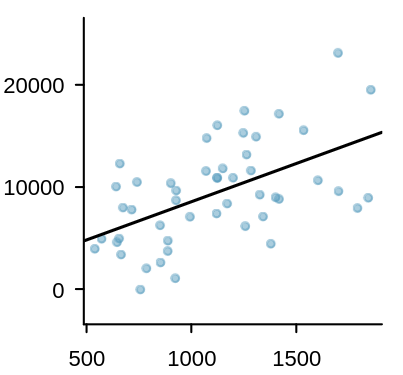
\includegraphics[width=.3\textwidth]{lin_reg_example.png}
    \caption{Exemplo de regressão linear. Fonte: \cite{openIntroStat}}
    \label{fig:lin_reg_example}
\end{figure}

Outra ferramenta que iremos utilizar neste artigo é o cálculo de correlação.
Segundo \cite{openIntroStat}, a correlação (\textit{R}) é uma medida com valor entre -1 e 1 que
indica o quão forte é a tendência linear entre as variáveis numéricas estudadas.
Quanto mais próximo de -1 for \textit{R}, maior é a força de correlação negativa.
Quanto mais próximo de 1 for \textit{R}, maior é a força de correlação positiva.
Por fim, quando mais próximo de 0 for \textit{R}, menor é a força de correlação entre os valores
estudados. A Figura~\ref{fig:correlation_example} mostra oito exemplos de correlação.

\begin{figure}[ht]
    \centering
    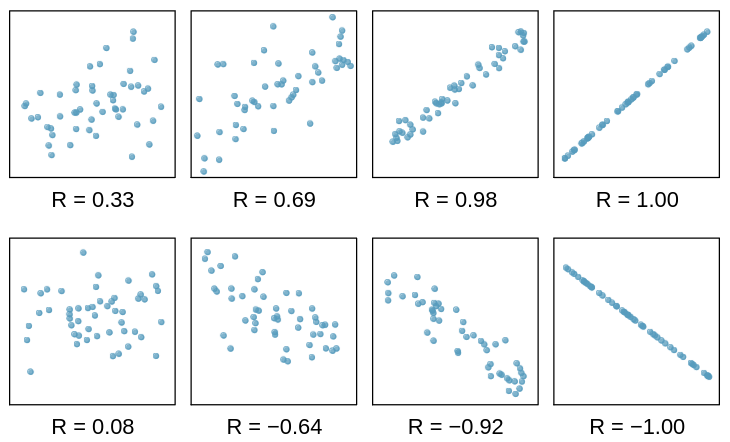
\includegraphics[width=.7\textwidth]{correlation_example.png}
    \caption{Exemplo correlação entre variáveis. Fonte: \cite{openIntroStat}}
    \label{fig:correlation_example}
\end{figure}

Com essas ferramentas estatísticas podemos verificar se existe alguma tendência entre os dados
estudados e, caso exista, qual a força da correlação entre elas.
É importante salientar que as tendencias e correlações calculadas não implicam em causalidade,
apenas nos dão insumos para uma análise mais criteriosa.

%%%%%%%%%%%%%%%%%%%%%%%%%%%%%%%%%%%%%%%%%%%%%%%%%%%%%%%%%%%%%%%%%%%%%%%%%%%%%%%%%%%%%%%%%%%%%%%%%%%%

\subsection{Ferramentas}

Diversas ferramentas foram utilizadas durante a obtenção, triagem e análise dos dados estudados
neste artigo.

O Bugzilla \cite{bugzilla} é um sistema de gerenciamento de defeitos que possibilita a organização,
categorização e discussão de defeitos reportados.
O projeto do qual os dados foram coletados utiliza o Bugzilla como sistema de gerenciamento de
defeitos. Nele existe um campo chamado ``\textit{Component}'' que é utilizado para indicar a qual
funcionalidade, do ponto de vista do usuário, aquele defeito é relativo, que será utilizado para
categorização dos defeitos neste presente estudo.

Os resultados de cobertura de código, no projeto estudado, são calculados pelo gcov \cite{gcov}, que
se trata de uma ferramente para geração de dados de cobertura de código para ser usada em conjunto
com o compilador \textbf{GCC} \cite{gcc}.

No projeto estudado, os testes, incluindo geração de dados de cobertura de código, são executados
automaticamente pelo Jenkins \cite{jenkins} (ferramenta para automatizações de integração contínua)
toda a vez que um novo \textit{commit} é submetido para revisão ou para o \textit{branch} principal.
Além dos resultados dos testes (sucesso ou falha) também são publicizados os dados de cobertura de
código calculados pelo gcov.

Na parte de triagem e análise dos dados, alguns \textit{scripts} em Python foram criados e estão
descritos em [REFERENCIAR APENDICES]. Nestes \textit{scripts} fora utilizadas as bibliotecas
(1) Plotly \cite{plotly}, uma biblioteca Python para geração de gráficos e (2) SciPy \cite{scipy},
uma biblioteca Python para auxílio de cálculos matemáticos e estatísticos.


%%%%%%%%%%%%%%%%%%%%%%%%%%%%%%%%%%%%%%%%%%%%%%%%%%%%%%%%%%%%%%%%%%%%%%%%%%%%%%%%%%%%%%%%%%%%%%%%%%%%
%%%%%%%%%%%%%%%%%%%%%%%%%%%%%%%%%%%%%%%%%%%%%%%%%%%%%%%%%%%%%%%%%%%%%%%%%%%%%%%%%%%%%%%%%%%%%%%%%%%%
%%%%%%%%%%%%%%%%%%%%%%%%%%%%%%%%%%%%%%%%%%%%%%%%%%%%%%%%%%%%%%%%%%%%%%%%%%%%%%%%%%%%%%%%%%%%%%%%%%%%

\section{Trabalhos Relacionados}

Em \cite{unitTestedCrash} os autores se propõe um estudo sobre a relação entre cobertura de código
a ocorrência de falhas, tentando traçar uma correlação entre os dois valores.
Como estudo de caso foram usados reportes de falhas em campo do projeto Eclipse.
O estudo coletou mais de 2 milhões de incidentes reportados e, após triagem de dados os autores
tinham em mãos mais de 126 mil reportes únicos do tipo \textit{stack trace}, que consiste em um tipo
de reporte de erro que contém informações como arquivo e linha de onde ocorreu a falha.

Em paralelo foram coletados dados da análise de cobertura de código do projeto em questão.
Como principal métrica de cobertura de código para a comparação foi utilizado a métrica de métodos
cobertos, que consiste em relacionar a quantidade de métodos existentes e quantos desses são
invocados nos testes.

Foi feita uma análise dos dados relacionando as falhas reportadas e a cobertura de código e a Tabela
\ref{tab:FalhasMetodosTeste} mostra os dados obtidos.
Do total de métodos analisados, 93,6\% não são testados 6,4\% dos testes são testados.
Analisando apenas os métodos que não possuem reportes de falhas relacionados essa proporção é de
93,5\% de métodos não testados, para 6,5\% de métodos testados.
Já quando analisamos métodos que possuem reportes de falhas relacionados essa proporção fica em
94,1\% de métodos não testados, para 5,9\% de métodos testados.

\begin{table}[ht]
\centering
\caption{Falhas de Métodos. Fonte: \cite{unitTestedCrash}}
\label{tab:FalhasMetodosTeste}
\begin{tabular}{|l|c|c|c|}
\hline
\multirow{2}{*}{Falha Reportada?} & \multicolumn{2}{c|}{Possui teste?} & \multirow{2}{*}{Total} \\ \cline{2-3}
                                  & Não   & Sim                        &       \\ \hline
Não                               & 7816  & 541                        & 8357  \\ \hline
Sim                               & 1097  &  69                        & 1166  \\ \hline
Total                             & 8913  & 619                        & 9523  \\ \hline
\end{tabular}
\end{table}

Com esse resultado o estudo conclui que não é possível afirmar que existe uma correlação entre
cobertura de código e uma menor quantidade de ocorrência de falhas. Os valores encontrados variam
marginalmente, apresentando um baixo valor de correlação.

Complementarmente, o artigo traz alguns itens a serem levados em conta.
Um deles é que o resultado foi utilizando apenas um projeto e tal projeto tem grandes proporções.
Os autores argumentam que o resultado não pode ser generalizado e pode vir a se diferente em outros
tamanhos de projeto.

O artigo \cite{coverageMetaAnalysis} traz uma revisão sistemática de outros trabalhos que analisam
uma possível correlação entre cobertura de código e efetividade de um conjunto de testes.
Para tal, os autores fizeram uma busca utilizando a ferramenta de busca Scopus para a seleção dos
trabalhos a serem estudados a fim de responder três questões de pesquisa:
\begin{enumerate}
    \item Quais evidências existem sobre a correlação entre cobertura de código e efetividade dos
          testes?

    \item Quais fatores impactam nessa relação?

    \item Qual métrica de cobertura de código é melhor para predizer a efetividade dos testes?
\end{enumerate}

O estudo descreve os termos de busca utilizados, além de duas etapas de filtragem de estudos que
foram necessárias para obter um material mais conciso para a revisão sistemática.
Após a primeira busca eles encontraram 427 resultados para a busca e, após os filtros retaram 33
estudos para serem analisados.

Segundo os autores, alguns estudos prévios apontavam que existe uma forte correlação entre cobertura
de código e efetividade dos testes.
Por outro lado alguns estudos indicavam que essa correlação era baixa ou até nula.

Como resultado desse artigo os autores argumentam que uma possível causa da não convergência dos
resultados dos estudos seja a falta de padronização entre os estudos, uma vez que os diversos
estudos revisados possuem abordagens diferentes de análise, além de casos de uso bem distintos entre
eles.
Para obter melhores resultados os autores recomendam atenção em alguns pontos que podem prejudicar
os resultados de estudos, tais como descartar projetos muito pequenos ou com uma cobertura
excessivamente baixa.
Outro ponto levantado pelos autores é uma lista de fatores que podem interferir na relação entre
cobertura de código e efetividade dos testes, como porcentagem de cobertura, testes que exercitem
tanto casos normais, quanto casos de exceção, tamanho do conjunto de testes, natureza das falhas,
complexidade do código, entre outros.


%%%%%%%%%%%%%%%%%%%%%%%%%%%%%%%%%%%%%%%%%%%%%%%%%%%%%%%%%%%%%%%%%%%%%%%%%%%%%%%%%%%%%%%%%%%%%%%%%%%%
%%%%%%%%%%%%%%%%%%%%%%%%%%%%%%%%%%%%%%%%%%%%%%%%%%%%%%%%%%%%%%%%%%%%%%%%%%%%%%%%%%%%%%%%%%%%%%%%%%%%
%%%%%%%%%%%%%%%%%%%%%%%%%%%%%%%%%%%%%%%%%%%%%%%%%%%%%%%%%%%%%%%%%%%%%%%%%%%%%%%%%%%%%%%%%%%%%%%%%%%%


\section{Metodologia de Pesquisa}

Essa pesquisa utilizou o método de estudo de caso e analisou os resultados por uma perspectiva
quantitativa.

Segundo \cite{estudoDeCasoYin}, ``você poderia utilizar o método de estudo de caso quando
deliberadamente quisesse lidar com condições contextuais - acreditando que elas poderiam ser
altamente pertinentes ao seu fenômeno de estudo''.
Nesse sentido o presente estudo utilizará como caso um sistema operacional embarcado em operação
desde 2015 em conjunto com suas métricas de cobertura de código e quantidade falhas encontradas.

Com base nos dados coletados, será feita uma análise quantitativa que, segundo
a definição de \cite{projetoDePesquisa}, utiliza raciocínio de causa e efeito, observação de dados,
teste de teorias, coleta de dados, entre outros instrumentos.

%%%%%%%%%%%%%%%%%%%%%%%%%%%%%%%%%%%%%%%%%%%%%%%%%%%%%%%%%%%%%%%%%%%%%%%%%%%%%%%%%%%%%%%%%%%%%%%%%%%%

\subsection{Delineamento de Pesquisa}

A presente pesquisa é de caráter quantitativo, visto que se pretende a traçar uma correlação entre
duas variáveis numéricas quantitativas -- percentual de cobertura de código e quantidade de falhas
reportadas.
Para descobrir de existe tal relação, os números encontrados serão submetidos a análises
estatísticas.

Para a coleta de dados, será feita uma pesquisa exploratória em um estudo de caso de um projeto
de sistema operacional.
Esse modelo de pesquisa é amplamente utilizado (\cite{coverageMetaAnalysis}, \cite{unitTestedCrash}
e \cite{coverageLargeScaleStudy}) em estudos do tipo, uma vez que a coleta de dados é precisa e de
fácil acesso, além de trazer uma representação muito próxima à realidade do caso estudado.

Apesar de a pesquisa ter um caráter quantitativo em seu objetivo principal, a utilização de métodos
qualitativos foram necessários em etapas intermediárias da pesquisa.
Durante a triagem dos dados obtidos, mas especificamente da classificação dos repositórios, foi
necessária a utilização da técnica de entrevistas para viabilizar tal classificação, uma vez que
esta não estava documentada.

%%%%%%%%%%%%%%%%%%%%%%%%%%%%%%%%%%%%%%%%%%%%%%%%%%%%%%%%%%%%%%%%%%%%%%%%%%%%%%%%%%%%%%%%%%%%%%%%%%%%

\subsection{Unidade de Análise} \label{Unidade de Análise}

A pesquisa ocorreu em uma empresa brasileira que projeta e desenvolve \textit{hardware} e
\textit{software}.
O enfoque do presente estudo será em um projeto específico de sistema operacional, abarcando todas
as funcionalidades desenvolvidas pela empresa dentro deste sistema operacional.

O sistema conta com 85 funcionalidades de usuário cadastradas e divididas em 316 repositórios
\textit{Git} ativos.
Uma funcionalidade de usuário, no contexto do presente artigo, é uma característica ou função
exercida pelo sistema operacional que seja percebida pelo usuário.
Desta forma, funções internas ao sistema operacional que não geram funcionalidade do ponto de vista
do usuário não são consideradas funcionalidade de usuário.
Cada funcionalidade pode ser implementada por 1 ou mais repositórios e cada repositório pode atender
0 ou mais funcionalidades de usuário. Um exemplo dessa representação pode ser visto na Figura
\ref{fig:features_repos}.

\begin{figure}[ht]
    \centering
    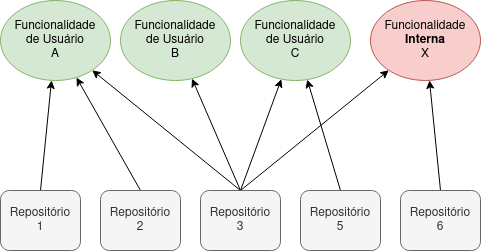
\includegraphics[width=.7\textwidth]{features_repos.png}
    \caption{Exemplo de relação entre repositórios de funcionalidades}
    \label{fig:features_repos}
\end{figure}

No contexto do projeto estudado, os testes de \textit{software} são divididos em duas categorias, de
acordo com o ambiente onde eles são executados.

A primeira categoria são os testes executados em ambientes de máquinas virtuais, ou
\textit{Virtual Machines} (VMs), em servidores especializados.
Essa categoria executa testes funcionais e estruturais de granularidade unitária e de componente,
além de calcular os dados de cobertura de código.
Esses testes são executados em dois momentos:
(1) sempre que um dado código é submetido para revisão, disparado pela submissão do código e
(2) diariamente, disparado por uma tarefa agendada do Jenkins.

A segunda categoria é a de testes executado no equipamento destino.
Nessa etapa existem vários equipamentos que terão seu sistema operacional atualizado com a versão
sobre teste e será executada uma bateria de testes a fim de testar as funcionalidades utilizando
os equipamentos reais e não mais máquinas virtuais.
Essa categoria de testes executa testes funcionais de granularidade de sistema, contendo o sistema
operacional com todos os componentes.

A Figura \ref{fig:pipeline_tests} mostra um resumo das etapas do desenvolvimento de software do
projeto em questão, enfatizando os momentos onde os testes ocorrem.
Analisando a figura, podemos perceber que os testes executados em VMs e disparados pela submissão
para revisão executam com base no código em revisão, já os testes periódicos disparados por tarefa
agendada o Jenkins executam com base no topo do repositório.

\begin{figure}[ht]
    \centering
    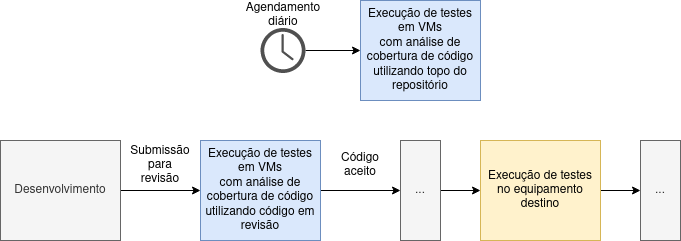
\includegraphics[width=1.0\textwidth]{pipeline_tests.png}
    \caption{Pipeline resumido da integração com enfoque na execução dos testes}
    \label{fig:pipeline_tests}
\end{figure}

Outro ponto importante a salientar é o contexto dos dados de cobertura de código.
Os dados gerados são específicos por repositório, ou seja, temos dados de cobertura de código dos
316 repositórios separadamente.

Uma vez que os testes em ambiente de máquinas virtuais são os testes que produzem dados de cobertura
de código, são esses testes que serão utilizados durante o presente estudo, deixando de fora os
testes executados nos equipamentos destino.
Os dados utilizados no estudo compreendem aos dados obtidos do topo dos repositórios, através da
execução periódica disparada pelo Jenkins.

Sobre a linguagem de programação adotada pelo projeto, a esmagadora maioria do código é escrito nas
linguagens C e C++.
A coleta de dados de cobertura de código foi feita em todos os repositórios que reportam cobertura
de códigos C e C++, sendo descartados códigos auxiliares escritos em outras linguagens, como Python
e Shell.

A coleta de dados de falhas reportadas compreende a todas as falhas relacionadas com o projeto
estudado e que não tenham sido corrigidas até o momento da pesquisa.
Isso inclui tanto falhas que ocorreram em campo, quanto falhas identificadas dentro da empresa, seja
por testes em equipamentos destino, testes de aceitação manual ou uso interno.
A decisão considerar apenas as falhas que não foram corrigidas se deu devido ao fato de que ao
considerar o conjunto de todas as falhas, estaríamos tendo interferência do histórico, o que poderia
interferir o resultado do estudo, uma vez que os dados de cobertura de código são relativos ao
momento atual.
E, por fim, a decisão de contabilizar todas as falhas, e não apenas as de campo, se deu devido à
compreensão de que os defeitos encontrados internamente não são menos relevantes, ou menos válidos
para o presente estudo, do que defeitos encontrados em campo.

%%%%%%%%%%%%%%%%%%%%%%%%%%%%%%%%%%%%%%%%%%%%%%%%%%%%%%%%%%%%%%%%%%%%%%%%%%%%%%%%%%%%%%%%%%%%%%%%%%%%

\subsection{Coleta de Dados}

O presente estudo se baseia em dados de duas naturezas distintas: (1) dados de falhas reportadas e
(2) dados de cobertura se código.
Ambos os dados foram coletados no dia 28/10/2023, representando o estado atual do projeto, tanto
do ponto de vista das falhas reportadas, quanto do ponto de vista da cobertura de código.
Uma vez que os dados coletados representam o estado o projeto na data de coleta, estes não podem
ser analisados sob uma óptica de evolução temporal do projeto, mas sim sob uma perspectiva de
``fotografia'' do projeto na data de coleta.

Apesar de ambos os dados terem sido coletados na mesma data, tais coletas foram feitas de formas
distintas, as quais serão apresentas nas sessões \ref{sec:falhasReportadas} e \ref{sec:cobertura}.

\subsubsection{Falhas Reportadas} \label{sec:falhasReportadas}

As falhas reportadas compreendem à quantidade de todas as falhas encontradas tanto externamente
(por clientes) quando internamente (por colaboradores).
O projeto estudado utiliza a ferramenta Bugzilla como ferramente gerenciadora de falhas tanto para
falhas descobertas internamente, quanto para falhas descobertas externamente, o que nos permite
acesso à toda a base de dados de falhas do projeto.
Contudo, o mesmo serviço do Bugzilla é utilizado na empresa para reportar falhas de outros projetos
e esse detalhe precisou ser levado em consideração no momento da formulação da busca.

O Bugzilla possui uma ferramenta de busca onde é possível listar bugs de acordo com um determinado
filtro de busca e a saída dessa busca pode ser de dois tipos: (1) HTML, onde é exibida uma interface
web contendo os resultados ou
(2) um arquivo do tipo CSV contendo uma linha para cada resultado encontrado, sendo as colunas
configuráveis via requisição HTML.
O formato escolhido foi o de arquivo CSV pois facilita a automação da triagem de dados.

A busca criada para selecionar a lista de falhas reportadas relacionadas ao projeto e que ainda não
forram solucionadas utilizou filtragem por dois campos do Bugzilla:

\begin{itemize}
    \item \textbf{Status}: Compreende ao estado atual do bug, que pode assumir diversos valores e
          se propõe a informar em qual fase de sua correção ele está, compreendendo desde as fases
          mais iniciais, como \textit{UNCONFIRMED}, que informa que não foi feita uma análise
          inicial, até as fases finais, como \textit{CLOSED}, onde o problema já foi resolvido e
          a solução foi aceita pelas equipes responsáveis pela aceitação.
          O termo escolhido para o filtro desse campo foi o de
          \textbf{``status!=(\textit{RESOLVED} OR \textit{CLOSED})''}.
          Ambos \textit{RESOLVED} e \textit{CLOSED} representam falhas reportadas que já tiveram sua
          correção integrada ao sistema operacional, porém \textit{RESOLVED} é um passo anterior,
          onde os desenvolvedores já fizeram as implementações, testes e integração, porém ainda
          não foi dado o aceite da correção, enquanto \textit{CLOSED} é o estado onde o aceite foi
          concedido.
          Essa escolha foi feita pois no fluxo de trabalho definido na empresa estudada as falhas
          são marcadas como \textit{CLOSED} apenas no fechamento de uma dada versão, sendo que elas
          podem já ter sido corrigidas, logo considerar ambos os termos nos traz uma fidelidade
          maior sobre os dados do projeto;

    \item \textbf{Project}: Compreende ao projeto em que foi encontrado esse problema. Existe um
          campo \textit{Project} específico para o projeto estudado, o qual vai ser utilizado na
          busca. Sendo assim, temos que o termo da busca de projeto é
          \textbf{``project==PROJETO''}, sendo PROJETO o nome que representa o projeto de sistema
          operacional estudado, mas não será divulgado por questões de sigilo empresarial.
\end{itemize}

Unindo os dois termos de busca, um que seleciona o estado da falha e o outro que seleciona o projeto
relativo à falha, temos o seguinte termo de busca:
\textbf{``(status!=(\textit{RESOLVED} OR \textit{CLOSED})) AND (project==PROJETO)''}.
Tal termo de busca tem por objetivo selecionar todas as falhas reportadas que ainda não tem solução
e que foram encontradas no projeto estudado.

Como resultado, o Bugzilla gera arquivo no formato CSV contendo 2 colunas:
(1) campo \textit{bugId}, que se trata de um número identificador do reporte de falha e
(2) campo \textit{component}, que informa em qual funcionalidade de usuário a falha foi encontrada.
O primeiro não terá utilidade no presente estudo, mas é um campo obrigatório nos reportes do
Bugzilla, já o segundo será utilizado para relacionar a quantidade de falhas reportadas com os
índices de cobertura de código.

Além do reporte de falhas reportadas no Bugzilla foi necessário obter a lista de todos os valores
possíveis do campo \textit{component}, o qual representa o conjunto de funcionalidade de usuário
disponíveis no sistema.
Essa lista é necessária para conhecermos todas as funcionalidades de usuário, um vez que a
funcionalidade pode não ter nenhuma falha reportada e, dessa forma, não apareceria no reporte de
falhas reportadas e ainda não corrigidas.
Essa lista foi utilizada para a estrita de um \textit{script}, o qual será descrito na sessão
\ref{sec:triagem}.

Com os dados obtidos é possível fazer a contagem de falhas reportadas por funcionalidade de cliente
e tal triagem dos dados será detalhada na sessão \ref{sec:triagem}.
Os dados resultantes da coleta de falhas reportadas não podem ser exibidos na íntegra por questões
de sigilo empresarial, porém foram compilados e anonimizados e serão exibidos na sessão
\ref{sec:resultados}.

\subsubsection{Cobertura de Código} \label{sec:cobertura}

A cobertura de código compreende à uma medida que indica a relação de quantidade de código testado
e código não testado.
O projeto estudado calcula tais dados utilizando a ferramenta gcov e executando os testes escritos
com auxílio do \textit{framework} Google Test, utilizado para desenvolvimento de testes de código
utilizando as linguagens C e C++.

Os dados de cobertura de código estavam inicialmente sendo disponibilizados através do
\textit{plugin} Cobertura \cite{jenkinsCobertura}, disponível do Jenkins
(Figura \ref{fig:pluginCobertura}), e as métricas de cobertura exportadas para o projeto são:
\begin{itemize}
    \item \textbf{Cobertura de Linhas}: Corresponde à quantidade de linhas de código testadas em
          relação ao total de linhas de código válidas do repositório;

    \item \textbf{Cobertura de Arquivos}: Corresponde ao total de arquivos contendo código executado
          nos testes em relação ao total de arquivos C e C++ do repositório;

    \item \textbf{Cobertura de Classes}: Corresponde ao total de classes acessadas nos testes em
          relação ao total de classes C e C++ do repositório;

    \item \textbf{Cobertura de Métodos}: Corresponde ao total de métodos chamados na execução dos
          testes em relação ao total de métodos C e C++ contidos no repositório.
          Um detalhe sobre este campo é que funções em códigos não orientados a objetos também são
          contabilizadas como métodos no contexto nesse reporte.
\end{itemize}

\begin{figure}[ht]
    \centering
    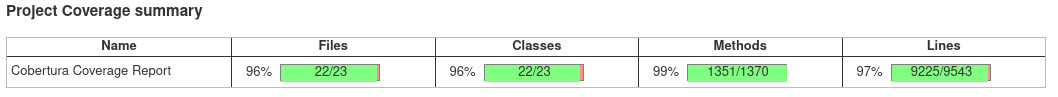
\includegraphics[width=1.0\textwidth]{cobertura.jpeg}
    \caption{Exemplo de exibição do \textit{plugin} Cobertura}
    \label{fig:pluginCobertura}
\end{figure}

Dentre todas métricas disponíveis a métrica de Cobertura de Linhas é a mais adequada.
Segundo \cite{coverageMetaAnalysis}, métricas mais genéricas, como cobertura de arquivos ou
cobertura de classes, são menos efetivas para relacionar a qualidade de código, ainda que tenham
validade.
No artigo os autores recomendam a utilização da métrica de Cobertura de Decisão, porém tal métrica
não está disponível atualmente no projeto e não pode ser utilizada.
Em vista disso, a métrica considerada mais adequada foi a de Cobertura de Linhas.

O \textit{plugin} Cobertura exibe dados utilizando uma interface web, o que dificulta a coleta de
dados, uma vez que seria necessário coletar manualmente os dados de cobertura de código dos 316
repositórios.
Para facilitar a coleta, o \textit{script} de geração de dados para o \textit{plugin} Cobertura
foi alterado a fim de gerar dados no formato de arquivos JSON, além do formato original, destinado
ao \textit{plugin} Cobertura.
Como resultado, o \textit{script} passou a gerar um arquivo JSON onde contendo uma lista de
repositórios e seus respectivos dados de cobertura de código, conforme mostra a Figura
\ref{fig:formatoJsonCoverage}.
Tal \textit{script} não pode ser exibido no presente artigo devido a questões relativas a sigilo
empresarial.

\begin{figure}[ht]
\caption{Exemplo de formatação do arquivo JSON gerado após alteração do \textit{script} de
geração de dados de cobertura de código.}
\label{fig:formatoJsonCoverage}
\begin{verbatim}
{
    "Nome do Repositório": {
        "lines-valid": <número de linhas válidas>,
        "line-rate": <taxa de cobertura>,
        "lines-covered": <número de linhas cobertas>
    },
    ...
}
\end{verbatim}
\end{figure}

Dessa forma teremos como resultado um arquivo JSON contendo todos os 316 repositórios e, para cada
um deles, seus respectivos dados de linhas válidas, linhas cobertas e taxa de cobertura.
Os dados de linhas válidas correspondem ao total de linhas de código C e C++, excluindo linhas que
não possuem execução, como linhas em branco, linhas de comentário e linhas de declarações de
métodos, por exemplo. Número de linhas cobertas corresponde ao total de linhas válidas que foram
executadas em pelo menos 1 teste. Por fim, a taxa de cobertura corresponde à divisão das linhas
cobertas pelas linhas válidas, conforme a Figura \ref{fig:formulaTaxaDeCobertura}.

\begin{figure}[ht]
\caption{Fórmula de cálculo de taxa de cobertura.}
\label{fig:formulaTaxaDeCobertura}
    \[ taxaDeCobertura = \frac{linhasCobertas}{linhasTotais} \]
\end{figure}

Uma vez que os dados de cobertura de código foram exportados via JSON, eles passaram a estar
disponíveis através do Jenkins.
Dessa forma é foi possível coletar os dados de cobertura por repositório através de
\textit{download} dos arquivos.
Cada repositório exporta seu dados diariamente, conforme descrito na sessão
\ref{Unidade de Análise}, e esses dados foram coletados através de requisições \textbf{wget}
em um terminal Linux com acesso ao Jenkins, sendo feita 1 requisição para cada um dos 316
repositórios.
Ao final, os dados foram organizados, de acordo com o descrito na sessão \ref{sec:triagem}.


%%%%%%%%%%%%%%%%%%%%%%%%%%%%%%%%%%%%%%%%%%%%%%%%%%%%%%%%%%%%%%%%%%%%%%%%%%%%%%%%%%%%%%%%%%%%%%%%%%%%

\subsection{Triagem e Análise de dados} \label{sec:triagem}

Antes de os dados serem analisados foi necessário um trabalho de triagem de dados, em especial da
porção de dados que compreende os dados de cobertura de código, a fim de organizá-los e
classificá-los.
Após a coleta, temos como insumo três dados distintos:
(1) um arquivo contendo dados de falhas reportadas,
(2) uma lista de funcionalidades de usuários cadastradas no Bugzilla e
(3) um arquivo contendo os dados de cobertura de código.

Os dados de falhas reportadas foram exportados em um arquivo CSV contendo a primeira linhas como
título das colunas e as demais sendo uma linha para cada falha reportada, com a filtragem de acordo
com o descrito na sessão \ref{sec:falhasReportadas}.
Em conjunto com a lista de funcionalidades de usuário foi criado um \textit{script} com o intuito
de contabilizar a quantidade de falhas reportadas em cada funcionalidade de usuário.
O \textit{script} está descrito no Apêndice [REFERENCIAR APENDICES] e produz um arquivo JSON
contendo uma lista de funcionalidades de usuário e, para cada uma delas, a quantidade de falhas
reportadas, contabilizadas através do arquivo CSV gerado pelo reporte do Bugzilla. Caso alguma
funcionalidade da lista de funcionalidades de usuário não tenha nenhuma falha associada no arquivo
CSV o valor de falhas reportadas para tal funcionalidade é considerado 0.

A Figura \ref{fig:formatoJsonBugs} mostra um exemplo da formatação do arquivo JSON gerada pelo
\textit{script} de contagem de falhas reportadas.
Na estrutura o campo \textbf{isComponent} indica se o elemento da lista é um \textit{component},
ou seja, se o elemento da lista é uma funcionalidade de usuário.
A necessidade desse campo será discutida mais adiante na presente sessão.
O outro campo presente na estrutura gerada é o campo \textbf{bugs}, o que indica a quantidade de
\textit{bugs} relativos àquele \textit{component}, isto é, a quantidade de falhas reportadas
relativas àquela funcionalidade de usuário.
Como resultado dessa primeira triagem obtivemos um arquivo no formado JSON contendo uma lista de
todas as funcionalidades de usuário e, dentro de cada elemento dessa lista, a informação de quantas
falhas reportadas estão relacionadas à dada funcionalidade.

\begin{figure}[ht]
\caption{Exemplo de formatação do arquivo JSON gerado após alteração do \textit{script} de contagem
de falhas reportadas, descrito em [REFERENCIAR APENDICES].}
\label{fig:formatoJsonBugs}
\begin{verbatim}
{
    "Nome da funcionalidade" : {
        "isComponent": true,
        "bugs": <number>
    },
    ...
}
\end{verbatim}
\end{figure}

Nesse ponto, temos de um lado a lista de funcionalidades e seus respectivos números de falhas
reportadas e de outro lado temos a lista de repositórios e seus respectivos dados de cobertura
de código.
O próximo passo foi relacionar os repositórios e as funcionalidades.
Para tal, foram feitas entrevistas com os líderes técnicos de todas as equipes.
A técnica de entrevista consiste em uma coleta de dados onde o entrevistador toma o entrevistado
como fonte de informação \cite{metodosPesquisaSocial}.
Uma vez que as informações de relacionamento entre repositórios e funcionalidade não estão
documentadas e em certos casos podem ser difusas, isto é, um repositório pode servir a mais de uma
funcionalidade de usuário, a entrevista com os líderes técnicos foi uma solução que atendeu as
necessidades da presente pesquisa.

O modelo de entrevista escolhido foi o modelo de entrevista focalizada que, de acordo com a
definição de \cite{metodosPesquisaSocial}, é uma entrevista pouco estruturada, onde o entrevistador
foca em um tema, no caso do estudo foi a relação entre repositórios e funcionalidades de usuário,
e permite que o entrevistado fale livremente, porém tentando manter o foco no tema definido.
As entrevistas foram feitas individualmente com 5 líderes técnicos, cobrindo todos os repositórios.
Para cada um deles a entrevista começou com o seguinte questionamento:

\begin{center}
\textit{Dado esses repositórios, a qual funcionalidade de usuários cada um deles pertence?}
\end{center}

Como resultado das entrevistas obtivemos os dados de funcionalidades de usuário e os dados de
cobertura de código unidos em um único arquivo em formato JSON, conforme o exemplo exibido na
Figura \ref{fig:formatoJsonFinal}.
Essa união foi feita manualmente durante as entrevistas.
Os campos \textbf{isComponent}, \textbf{bugs}, \textbf{lines-valid}, \textbf{line-rate},
\textbf{lines-covered} continuam com o mesmo significado dos passos anteriores, porém aqui podemos
ver um novo campo: \textbf{reposCoverage}.
O campo \textbf{reposCoverage} é um elemento que contém uma lista com todos os repositórios
referentes à funcionalidade no qual este elemento está inserido, bem como os dados de cobertura de
código destes repositórios.
Além disso, foram criados outros agrupamentos de repositórios que não fazem referência a uma
funcionalidade específica e, por esse motivo, foram marcadas como \textbf{false} no campo
\textbf{isComponent}.
Essa marcação facilita a compilação de dados feita por alguns \textit{scripts} que serão detalhados
adiante nesta mesma sessão.

\begin{figure}[ht]
\caption{Exemplo de formatação do arquivo JSON junção manual dos dados de falhas reportadas por
funcionalidade e dados de cobertura de código por repositório.}
\label{fig:formatoJsonFinal}
\begin{verbatim}
{
    "Nome da funcionalidade" : {
        "isComponent": true,
        "bugs": <number>,
        "reposCoverage": {
            "nome-do-repositório-x": {
                "lines-valid": <number>,
                "line-rate": <number>,
                "lines-covered": <number>
            },
            ...
        }
    },
    "Outras divisões": {
        "isComponent": false,
        "reposCoverage": {
            "nome-do-repositório-y": {
                "lines-valid": <number>,
                "line-rate": <number>,
                "lines-covered": <number>
            },
            ...
        }
    },
    ...
}
\end{verbatim}
\end{figure}

Após a integração dos dados, tivemos repositórios sendo classificados de 3 formas diferentes:
\begin{itemize}
    \item \textbf{Repositórios que não estão em campo}:
          são repositórios que não foram entreges no sistema operaciona, ou foram obsoletados em
          algum momento. Tais repositórios foram agrupados em uma divisão chamada
          \textbf{\textit{Not In Field}}, que reúne os repositórios que ainda não estão ou não estão
          mais sendo utilizados e, por esse motivo, não possuem falhas reportadas relativas a eles.
          Esses repositórios foram desconsiderados nas análises estatísticas;

    \item \textbf{Repositórios de sistema}:
          são repositórios que servem a mais de uma funcionalidade simultaneamente.
          Estes foram agrupados em uma divisão chamada \textbf{\textit{System repos}}.
          Uma vez que esses repositórios não foram relacionados a um funcionalidade específica, eles
          foram descartados de grande parte das análises estatísticas, mas não todas, sendo usado em
          alguns cálculos de média e mediana;

    \item \textbf{Repositórios de funcionalidade}:
          são repositórios que servem a apenas uma funcionalidade de usuário, sendo colocados dentro
          do elemento referente a sua funcionalidade.
\end{itemize}

O último passo referente ao tratamento inicial dos dados, antes da análise dos mesmo, foi a
a ofuscação de dados.
Os dados originais contém os nomes reais das funcionalidades e repositórios e eles foram ofuscados
por questões de sigilo empresarias.
O \textit{script} responsável pela ofuscação de dados está descrito no Apêndice [REFERENCIAR APENDICES]
e ele é responsável por receber como entrada o arquivo JSON com nomes originais e gerar um novo
arquivo JSON com nomes genéricos, seguindo o seguinte padrão:
\textbf{Component\_\textless número\textgreater} e
\textbf{Repository\_\textless número\textgreater}.
Além das questões de sigilo empresarial, a ofuscação dos dados permite-nos uma análise de dados
excluindo vieses, uma vez que não é possível distinguir funcionalidades e repositórios.

O passo seguinte à triagem de dados foi a análise dos mesmos.
Tendo como base um arquivo JSON contendo todos os dados de falhas reportadas divididas por
funcionalidade e seus respectivos repositórios contendo dados de cobertura de código, foi possível
analisar os dados e gerar os resultados estatísticos.

Como objetivo principal deste estudo temos a seguinte questão de pesquisa:
``Existe correlação entre cobertura de código e qualidade de \textit{software} de um sistema
operacional embarcado, sendo cobertura de linhas a métrica de cobertura de código e número de falhar
reportadas a métrica de qualidade de \textit{software}?'' e para respondê-la podemos recorrer a
cálculos estatísticos.
Nesse sentido, o primeiro passo foi gerar um gráfico de bolhas (veja exemplo na
Figura \ref{fig:bubble_example}) com o eixo x sendo a taxa de cobertura de código, o eixo y a
quantidade de falhas reportadas e cada bolha sendo uma funcionalidade, onde o tamanho da bolha
indica a quantidade de linhas de código, representando o tamanho, em linhas da funcionalidade.
Esse tipo de gráfico permite termos uma visualização gráfica inicial dos dados.

\begin{figure}[ht]
    \centering
    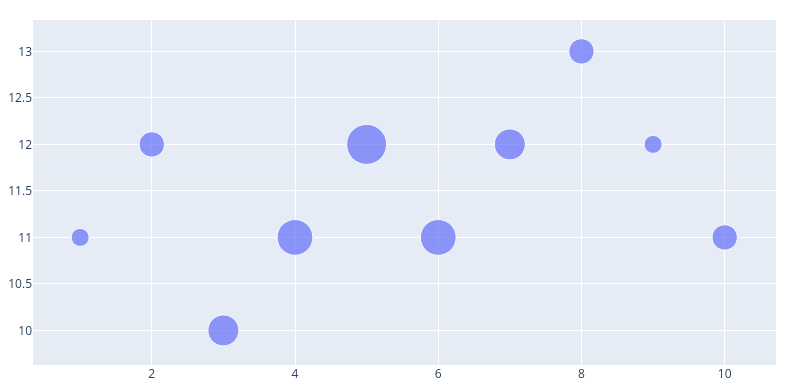
\includegraphics[width=0.8\textwidth]{bubble_example.png}
    \caption{Exemplo de gráfico de bolhas \cite{plotly}.}
    \label{fig:bubble_example}
\end{figure}

De forma complementar, foi utilizado uma linha de regressão linear adicional ao gráfico de bolhas
(veja exemplo na Figura \ref{fig:lin_reg_example}).
Segundo \cite{openIntroStat}, modelos de regressão linear podem ser usados para previsões com base
em dados de duas variáveis numéricas.
No caso estudado as variáveis são taxa de cobertura de código e número de falhas reportadas.
Para a geração do gráfico contendo as bolhas e a linha de regressão linear foi utilizado a
biblioteca Plotly en sua versão para a linguagem Python \cite{plotly}.
Através dessa biblioteca é possível gerar os gráficos de forma fácil utilizando o método de Mínimos
Quadrados Ordinários, ou \textit{Ordinary Least Squares} (OLS), em inglês.

\begin{figure}[ht]
    \centering
    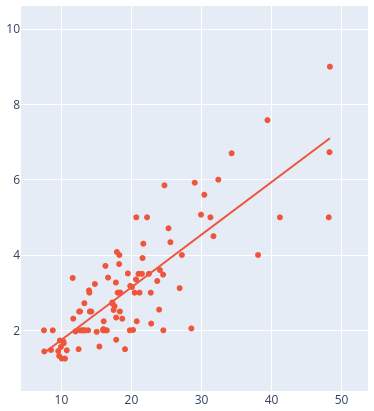
\includegraphics[width=0.5\textwidth]{linear_regression_example.png}
    \caption{Exemplo de gráfico de bolhas com linha de regressão linear \cite{plotly}.}
    \label{fig:lin_reg_example}
\end{figure}

A geração dos gráficos foi feita através do \textit{script} descrito no Apêndice [REFERENCIAR APENDICES].
Note que, como exibido na Figura \ref{fig:formatoJsonFinal}, o JSON possui os dados de cobertura de
código por repositório, porém precisamos dos dados por funcionalidade.
Para resolver essa questão, o \textit{script} gerador do gráfico também faz um pré-processamento
dos dados, somando os dados de cobertura de código de todos os repositórios de uma mesma
funcionalidade (veja fórmula na Figura \ref{fig:formulaTaxaDeCoberturaComponent}), obtendo assim os
dados de cobertura de código de uma funcionalidade.

\begin{figure}[ht]
\caption{Fórmula de cálculo de taxa de cobertura de uma funcionalidade de usuário.}
\label{fig:formulaTaxaDeCoberturaComponent}
\begin{center}
    $taxaDeCoberturaFuncionalidade = {\sum_{i=a}^{N} linhasCobertas_i \over \sum_{i=a}^{N} linhasTotais_i}$, sendo
    \textbf{a} e \textbf{N} o primeiro e último repositório referente à funcionalidade, respectivamente
\end{center}
\end{figure}

Com o gráfico de bolhas e regressão linear já é possível concluir se existe ou não correlação entre
as variáveis estudadas, porém ainda não é possível quantificar a força dessa correlação.
Para tal o script descrito no Apêndice [REFERENCIAR APENDICES] utiliza a biblioteca ScyPy
\cite{scipy} para fazer o cálculo de correlação $R$ que, segundo \cite{scipy} segue a fórmula
descrita na Figura \ref{fig:formulaCorrelacao}.
Com o valor resultante do cálculo é possível mensurar se a correlação é fraca ou forte e se é
positiva ou negativa \cite{openIntroStat}.

\begin{figure}[ht]
\caption{Fórmula da correlação de Pearson. Fonte: \cite{scipy}}
\label{fig:formulaCorrelacao}
\begin{center}
    $R = {\sum(x - m_x)(y - m_y) \over \sqrt{\sum(x - m_x)^2 \sum(y - m_y)^2}}$
\end{center}
\end{figure}

Por fim, alguns cálculos estatísticos auxiliares foram utilizados em algumas análises minoritárias,
como o cálculos de média aritmétca (veja Figura \ref{fig:formulaMedia}) e mediana, a fim de capturar
tendências de valores para grupos de repositórios.

\begin{figure}[ht]
\caption{Fórmula da média. Fonte: ENCONTRAR UMA FONTE}
\label{fig:formulaMedia}
\begin{center}
    $M = {\sum_{i=1}^{N} x_i \over N}$
\end{center}
\end{figure}

%%%%%%%%%%%%%%%%%%%%%%%%%%%%%%%%%%%%%%%%%%%%%%%%%%%%%%%%%%%%%%%%%%%%%%%%%%%%%%%%%%%%%%%%%%%%%%%%%%%%

\subsection{Limitações Apresentadas}

Nesta sessão serão apresentados alguns pontos de limitação e possíveis vulnerabilidades do presente
estudo, a fim de ressaltar pontos de atenção durante a análise dos resultados obtidos.

No estudo de caso apresentado neste artigo temos uma análise de 85 funcionalidades distribuídas em
316 repositórios distintos.
Ainda que o $N$ amostral tenha um tamanho relevante, ele apresenta algumas vulnerabilidades, as
quais discutiremos neste parágrafo.
Todo o código analisado data de diversos períodos, deste meados de 2013, quando o projeto começou a
ser implementado até o ano de 2023, quando o presente estudo foi feito.
Durante todo esse período o projeto contou com dezenas de equipes diferentes e centenas de
desenvolvedores.
Apesar da grande pluralidade de estilos de desenvolvimento, o projeto sempre esteve dentro da mesma
empresa, com a mesma cultura de desenvolvimento, as mesmas linguagens de desenvolvimento e, por fim,
atendendo um perfil de cliente que foi pouco modificado durante a vida do projeto.
Estas constantes podem gerar um certo viés que imponha os resultados obtidos, sem que estes sejam
genéricos o suficiente para que sejam comparáveis com outros projetos.
Além disso, as falhas são reportadas por um perfil de usuário específico, o que pode fazer com que
os valores de falhas reportadas não sejam comparáveis com os valores de outros projetos.
A fim de minimizar essas limitações mais estudos são necessários, envolvendo projetos de tamanhos,
perfis e tecnologias distintas.

Outro ponto que pode ser considerado como uma limitação é a métrica de cobertura de código
utilizada.
Neste estudo utilizamos a métrica de cobertura de linhas de código, porém esta pode não ser a
métrica mais adequada para a correlação entre cobertura de código e falhas reportadas.
Existem outras métricas de cobertura de código, como cobertura de decisão, que poderiam ter sido
utilizadas em conjunto com a métrica de cobertura de linhas, a fim de termos uma maior base de dados
para análise, o que poderia gerar conclusões mais precisas a respeito da existência ou não da
correlação e de qual a melhor métrica a se utilizar para mensurar tal correlação.

Durante a triagem dos dados foi necessário traçar a relação entre repositórios e funcionalidades
de usuário.
Tal correlação pode ser bem difusa.
Alguns repositórios podem servir a mais de uma funcionalidade em proporções diferentes, bem como
podem existir funcionalidades de usuário muito semelhantes e a classificação das falhas pode ficar
dificultada.
Essas questões de classificação, tanto das falhas, quanto dos repositórios, são feitas por pessoas
e, devido à característica difusa, podem ter sido classificadas de forma não adequada.
Essas falhas de classificação podem gerar alterações tanto positivas, quanto negativas nos
resultados, o que nos traz mais um ponto de atenção.
Uma vez que as classificações são feitas qualitativamente, elas estão sujeitas a erro humano e podem
representar uma menor precisão dos resultados.

Alguns dos repositórios foram classificados como \textbf{repositórios de sistema}.
Essa denominação denota repositórios que não pertencem a apenas uma funcionalidade, atendendo a duas
ou mais funcionalidades simultaneamente.
Tais repositórios não foram considerados nos cálculos e análises, uma vez que não seria possível
atribuir seus dados de cobertura a uma só funcionalidade.
Essa abordagem deixa de fora alguns repositórios, o que pode impactar nos resultados, visto que tais
repositórios podem ser responsáveis por falhas das funcionalidades, mas não são contabilizados nas
estatísticas de cobertura de código da funcionalidade.
Para tornar a abordagem mais precisa, seria necessário obter mais informações sobre a influência
de \textbf{repositórios de sistema} nas funcionalidades as quais eles interferem.

Da perspectiva dos testes utilizados como base das informações de cobertura de código, podemos
observar mais uma limitação metodológica.
O conjunto de testes que geram informações de cobertura de código é um subconjunto do total de
testes existentes.
Os testes que executam no equipamento destino não geram estatísticas de cobertura de código pois
a ferramenta \textbf{gcov} não está embarcada no equipamento.
Cada funcionalidade pode ter uma proporção diferente de testes com e sem estatísticas de cobertura
de código, o que pode interferir na comparação entre funcionalidades.

Tais limitações e vulnerabilidades não invalidam o resultado do estudo, porém indicam pontos que
devem ser observado durante a leitura e interpretação dos resultados.
De maneira geral, podemos compreender que os resultados observados são válidos no contexto do
projeto estudado e durante o período observado, não sendo garantida uma generalização dos resultados
para outros projetos.
Apesar disso, os dados obtidos podem ser utilizados como indícios quando analisados em conjunto com
mais pesquisas do mesmo tema, ou de pesquisas mais abrangentes.
Além disso, é importante ressaltar que o presente artigo se propões a um estudo de
\textbf{correlação} e, com as informações que temos no contexto estrito deste estudo, não é possível
garantir uma correlação causal.


%%%%%%%%%%%%%%%%%%%%%%%%%%%%%%%%%%%%%%%%%%%%%%%%%%%%%%%%%%%%%%%%%%%%%%%%%%%%%%%%%%%%%%%%%%%%%%%%%%%%
%%%%%%%%%%%%%%%%%%%%%%%%%%%%%%%%%%%%%%%%%%%%%%%%%%%%%%%%%%%%%%%%%%%%%%%%%%%%%%%%%%%%%%%%%%%%%%%%%%%%
%%%%%%%%%%%%%%%%%%%%%%%%%%%%%%%%%%%%%%%%%%%%%%%%%%%%%%%%%%%%%%%%%%%%%%%%%%%%%%%%%%%%%%%%%%%%%%%%%%%%


\section{Resultados} \label{sec:resultados}

Esta sessão tem como objetivo apresentar os resultados obtidos no estudo.

Todos os resultados descritos nesta sessão se baseiam no arquivo contido no Apêndice
[REFERENCIAR APENDICES], que consiste em um arquivo no formato JSON contendo todos os números de
falhas reportadas e cobertura de código, bem como os relacionamentos entre repositórios e
funcionalidades de usuário, conforme descrito na sessão \ref{sec:triagem}.

Após a triagem dos dados coletados, podemos ver a lista de falhas reportadas por funcionalidade
conforme descrito na Tabela \ref{tab:falhasReportadas}.

%\begin{table}[ht]
%\centering
%\caption{Lista de funcionalidades, quantidade de falhas reportadas e quantidade de repositórios.}
%\label{tab:falhasReportadas}
%\begin{tabular}{|l|c|c||l|c|c|}
%\hline
%Funcionalidade      & Falhas & Repositórios & Funcionalidade      & Falhas & Repositórios \\ \hline
%Funcionalidade\_001 & 7      & 2            & Funcionalidade\_044 & 6      & 1 \\ \hline
%Funcionalidade\_002 & 0      & 0            & Funcionalidade\_045 & 2      & 1 \\ \hline
%Funcionalidade\_003 & 0      & 0            & Funcionalidade\_046 & 6      & 2 \\ \hline
%Funcionalidade\_004 & 0      & 0            & Funcionalidade\_047 & 26     & 4 \\ \hline
%Funcionalidade\_005 & 0      & 0            & Funcionalidade\_048 & 5      & 2 \\ \hline
%Funcionalidade\_006 & 0      & 0            & Funcionalidade\_049 & 12     & 3 \\ \hline
%Funcionalidade\_007 & 0      & 0            & Funcionalidade\_050 & 4      & 2 \\ \hline
%Funcionalidade\_008 & 0      & 1            & Funcionalidade\_051 & 2      & 2 \\ \hline
%Funcionalidade\_009 & 0      & 0            & Funcionalidade\_052 & 2      & 1 \\ \hline
%Funcionalidade\_010 & 4      & 0            & Funcionalidade\_053 & 7      & 5 \\ \hline
%Funcionalidade\_011 & 108    & 26           & Funcionalidade\_054 & 22     & 7 \\ \hline
%Funcionalidade\_012 & 8      & 0            & Funcionalidade\_055 & 2      & 2 \\ \hline
%Funcionalidade\_013 & 1      & 0            & Funcionalidade\_056 & 10     & 2 \\ \hline
%Funcionalidade\_014 & 14     & 0            & Funcionalidade\_057 & 152    & 12 \\ \hline
%Funcionalidade\_015 & 2      & 0            & Funcionalidade\_058 & 1      & 19 \\ \hline
%Funcionalidade\_016 & 2      & 0            & Funcionalidade\_059 & 3      & 1 \\ \hline
%Funcionalidade\_017 & 6      & 0            & Funcionalidade\_060 & 13     & 4 \\ \hline
%Funcionalidade\_018 & 4      & 5            & Funcionalidade\_061 & 1      & 2 \\ \hline
%Funcionalidade\_019 & 36     & 3            & Funcionalidade\_062 & 3      & 1 \\ \hline
%Funcionalidade\_020 & 47     & 3            & Funcionalidade\_063 & 10     & 3 \\ \hline
%Funcionalidade\_021 & 1      & 1            & Funcionalidade\_064 & 6      & 7 \\ \hline
%Funcionalidade\_022 & 3      & 0            & Funcionalidade\_065 & 3      & 2 \\ \hline
%Funcionalidade\_023 & 23     & 0            & Funcionalidade\_066 & 2      & 2 \\ \hline
%Funcionalidade\_024 & 9      & 0            & Funcionalidade\_067 & 4      & 6 \\ \hline
%Funcionalidade\_025 & 2      & 0            & Funcionalidade\_068 & 9      & 1 \\ \hline
%Funcionalidade\_026 & 2      & 0            & Funcionalidade\_069 & 1      & 5 \\ \hline
%Funcionalidade\_027 & 3      & 0            & Funcionalidade\_070 & 2      & 2 \\ \hline
%Funcionalidade\_028 & 0      & 8            & Funcionalidade\_071 & 6      & 5 \\ \hline
%Funcionalidade\_029 & 0      & 1            & Funcionalidade\_072 & 3      & 5 \\ \hline
%Funcionalidade\_030 & 0      & 2            & Funcionalidade\_073 & 2      & 1 \\ \hline
%Funcionalidade\_031 & 0      & 4            & Funcionalidade\_074 & 23     & 1 \\ \hline
%Funcionalidade\_032 & 0      & 1            & Funcionalidade\_075 & 4      & 2 \\ \hline
%Funcionalidade\_033 & 0      & 4            & Funcionalidade\_076 & 7      & 1 \\ \hline
%Funcionalidade\_034 & 0      & 2            & Funcionalidade\_077 & 2      & 4 \\ \hline
%Funcionalidade\_035 & 2      & 0            & Funcionalidade\_078 & 3      & 2 \\ \hline
%Funcionalidade\_036 & 0      & 2            & Funcionalidade\_079 & 13     & 7 \\ \hline
%Funcionalidade\_037 & 12     & 1            & Funcionalidade\_080 & 12     & 4 \\ \hline
%Funcionalidade\_038 & 5      & 3            & Funcionalidade\_081 & 10     & 5 \\ \hline
%Funcionalidade\_039 & 1      & 2            & Funcionalidade\_082 & 9      & 1 \\ \hline
%Funcionalidade\_040 & 7      & 2            & Funcionalidade\_083 & 1      & 3 \\ \hline
%Funcionalidade\_041 & 16     & 2            & Funcionalidade\_084 & 2      & 1 \\ \hline
%Funcionalidade\_042 & 3      & 2            & Funcionalidade\_085 & 0      & 1 \\ \hline
%Funcionalidade\_043 & 5      & 2            & & & \\ \hline
%\end{tabular}
%\end{table}

Observando a tabela é possível perceber que as funcionalidade possuem um número variado de falhas
reportadas e repositórios repositórios relacionados.
Dado que o objetivo do presente estudo é traçar uma correlação entre cobertura de código de número
de falhas reportadas, as funcionalidades que não possuem nenhum repositório relacionado foram
descartadas, uma vez que são os repositórios que possuem os dados de cobertura de código.

Os casos de funcionalidades sem repositórios relacionados ocorrem quando a funcionalidade é
implementada utilizando apenas repositórios de sistema, ou seja, apenas repositórios quem atendem a
mais de uma funcionalidade.
Dessa forma não é possível atribuir a cobertura de código à funcionalidade, seguindo as regras
estabelecidas na sessão de \ref{sec:triagem}.

Após o descarte das funcionalidade sem repositórios, restaram 64 funcionalidades, conforme
Tabela \ref{tab:falhasReportadasClean}.
Apenar dos resultados filtrados, ainda é necessário relacionar os dados de funcionalidade com os
dados de cobertura de código.

%\begin{table}[ht]
%\centering
%\caption{Lista de funcionalidades, quantidade de falhas reportadas e quantidade de repositórios.
%Excluindo funcionalidade sem repositórios.}
%\label{tab:falhasReportadasClean}
%\begin{tabular}{|l|c|c||l|c|c|}
%\hline
%Funcionalidade      & Falhas & Repositórios & Funcionalidade      & Falhas & Repositórios \\ \hline
%Funcionalidade\_001 &   7    & 2            & Funcionalidade\_054 &  22    & 7 \\ \hline
%Funcionalidade\_008 &   0    & 1            & Funcionalidade\_055 &   2    & 2 \\ \hline
%Funcionalidade\_011 & 108    & 26           & Funcionalidade\_056 &  10    & 2 \\ \hline
%Funcionalidade\_018 &   4    & 5            & Funcionalidade\_057 & 152    & 1 \\ \hline
%Funcionalidade\_019 &  36    & 3            & Funcionalidade\_058 &   1    & 19 \\ \hline
%Funcionalidade\_020 &  47    & 3            & Funcionalidade\_059 &   3    & 1 \\ \hline
%Funcionalidade\_021 &   1    & 1            & Funcionalidade\_060 &  13    & 4 \\ \hline
%Funcionalidade\_028 &   0    & 8            & Funcionalidade\_061 &   1    & 2 \\ \hline
%Funcionalidade\_029 &   0    & 1            & Funcionalidade\_062 &   3    & 1 \\ \hline
%Funcionalidade\_030 &   0    & 2            & Funcionalidade\_063 &  10    & 3 \\ \hline
%Funcionalidade\_031 &   0    & 4            & Funcionalidade\_064 &   6    & 7 \\ \hline
%Funcionalidade\_032 &   0    & 1            & Funcionalidade\_065 &   3    & 2 \\ \hline
%Funcionalidade\_033 &   0    & 4            & Funcionalidade\_066 &   2    & 2 \\ \hline
%Funcionalidade\_034 &   0    & 2            & Funcionalidade\_067 &   4    & 6 \\ \hline
%Funcionalidade\_036 &   0    & 2            & Funcionalidade\_068 &   9    & 1 \\ \hline
%Funcionalidade\_037 &  12    & 1            & Funcionalidade\_069 &   1    & 5 \\ \hline
%Funcionalidade\_038 &   5    & 3            & Funcionalidade\_070 &   2    & 2 \\ \hline
%Funcionalidade\_039 &   1    & 2            & Funcionalidade\_071 &   6    & 5 \\ \hline
%Funcionalidade\_040 &   7    & 2            & Funcionalidade\_072 &   3    & 5 \\ \hline
%Funcionalidade\_041 &  16    & 2            & Funcionalidade\_073 &   2    & 1 \\ \hline
%Funcionalidade\_042 &   3    & 2            & Funcionalidade\_074 &  23    & 1 \\ \hline
%Funcionalidade\_043 &   5    & 2            & Funcionalidade\_075 &   4    & 2 \\ \hline
%Funcionalidade\_044 &   6    & 1            & Funcionalidade\_076 &   7    & 1 \\ \hline
%Funcionalidade\_045 &   2    & 1            & Funcionalidade\_077 &   2    & 4 \\ \hline
%Funcionalidade\_046 &   6    & 2            & Funcionalidade\_078 &   3    & 2 \\ \hline
%Funcionalidade\_047 &  26    & 4            & Funcionalidade\_079 &  13    & 7 \\ \hline
%Funcionalidade\_048 &   5    & 2            & Funcionalidade\_080 &  12    & 4 \\ \hline
%Funcionalidade\_049 &  12    & 3            & Funcionalidade\_081 &  10    & 5 \\ \hline
%Funcionalidade\_050 &   4    & 2            & Funcionalidade\_082 &   9    & 1 \\ \hline
%Funcionalidade\_051 &   2    & 2            & Funcionalidade\_083 &   1    & 3 \\ \hline
%Funcionalidade\_052 &   2    & 1            & Funcionalidade\_084 &   2    & 1 \\ \hline
%Funcionalidade\_053 &   7    & 5            & Funcionalidade\_085 &   0    & 1 \\ \hline
%\end{tabular}
%\end{table}

A Figura \ref{fig:cc_bugs_geral} mostra um gráfico de bolhas que dispõe a relação entre taxa de
cobertura de linhas (eixo $x$) e a quantidade de falhas reportada (eixo $y$).
O tamanho das bolhas represeta a quantidade de linhas totais da funcionalidade, porém a proporção
não é linear.

\begin{figure}[ht]
    \centering
    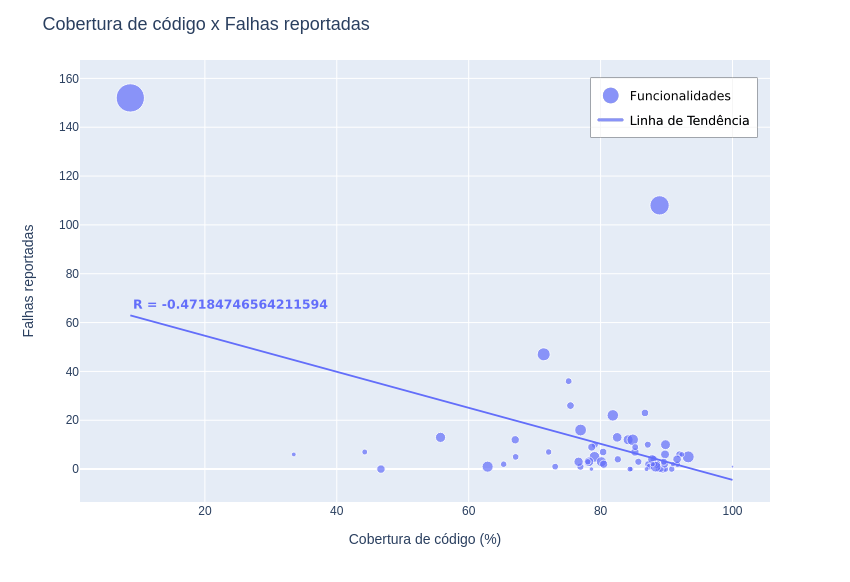
\includegraphics[width=1.0\textwidth]{cc_bugs_geral.png}
    \caption{Cobertura de código versus falhas reportadas. Gráfico inclui todos as funcionalidades
com pelo menos 1 repositório associado.}
    \label{fig:cc_bugs_geral}
\end{figure}

Em um primeiro momento é possível observar uma grande quantidade de funcionalidades no quadrande
inferior direito, o que representa uma concentração de funcionalidades com alta cobertura de código
e baixo número de falhas reportadas.
À medida que a cobertura de código diminui, a variabilidade da quantidade de falhas reportadas tende
a aumentar, formando uma espécie de cone que diminui sua variabilidade no eixo $y$ à medida que
a cobertura de código, representada no eixo $x$ aumenta, tendendo a $y = 0$.

A linha de tendência, calculada atravé da regressão linear por Mínimos Quadrados Ordinários,
também corrobora a tese de que existe uma correlação.
A linha indica uma correlação negativa entre os valores de cobertura de código e falhas reportadas,
isto é, a quantidade de falhas reportadas tende a ser menor à medida que acobertura de código
aumenta.
Além da linha de tendência, o coeficiente de correlação também indica uma correlação sustentável.
O coeficiente de correlação $R \approx 0,49$ mostra que a correlação não é nula ($R = 0$), mas
também não é perfeita ($R = -1$ ou $R = 1$), ficando no meio do caminho entre ambos.

Outro ponto de interessande de se notar são as duas funcionalidades com as maiores quantidades de
falhas reportadas.
Ambas as funcionalidades tem grande quantidade de código, indicado pelos tamanhos de suas
respectivas bolhas, o que pode indicar que o tamanho da funcionalidade, medido em linhas de código,
também possa vir a ser um indicativo de quantidade de falhas reportadas.
Contudo, uma vez que o presente estudo não se destina a estudar a relação do tamanho de código com
a quantidade de falhas reportadas, não vamos nos aprofundar nesse tema.

Outra visualização possível é a cobertura de código versus falhas reportadas excluindo
funcionalidades sem bugs reportados (Figura \ref{fig:cc_bugs_com_bugs}).
O objetivo dessa visualizaçãoé incluir apenas funcionalidades que se tem certeza que foram
utilizadas, uma vez que não é possível descobrir uma falha sem a utilização da funcionalidade.
Observando a Figura \ref{fig:cc_bugs_com_bugs} podemos ver que a tendência permanece muito próxima
à Figura \ref{fig:cc_bugs_geral}, mantendo uma inclinação próxima na linha de tendência e com um
$R \approx 0,47$, valor muito próximo ao $R \approx 0,49$ da Figura \ref{fig:cc_bugs_geral}.
Isso indica que ambas as visualizações são equivalentes, do ponto de vista estatístico.

\begin{figure}[ht]
    \centering
    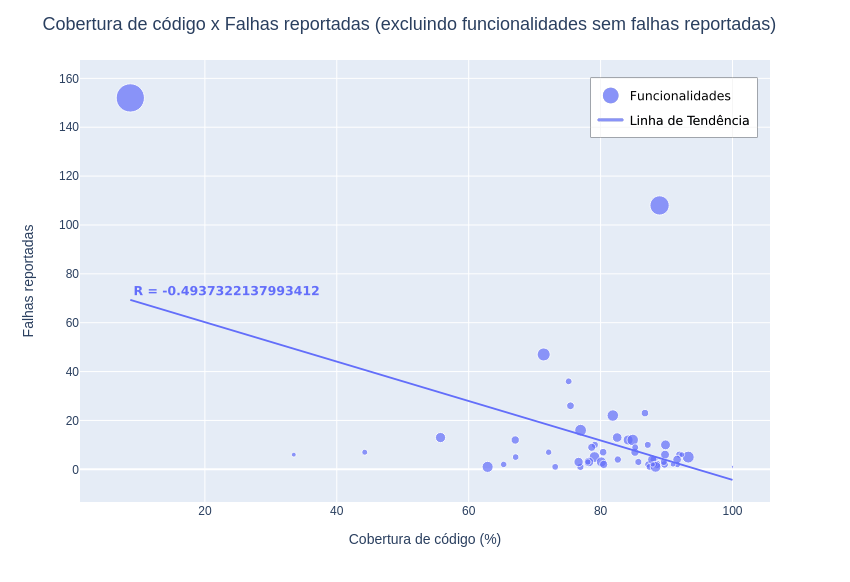
\includegraphics[width=1.0\textwidth]{cc_bugs_com_bugs.png}
    \caption{Cobertura de código versus falhas reportadas. Gráfico exclui funcionalidades sem
falhas reportadas.}
    \label{fig:cc_bugs_com_bugs}
\end{figure}

Analisando os dados da Tabela [REFERENCIAR ALGUMA TABELA], podemos separar as funcionalidades em
dois grandes grupos:
(1) o grupo das funcionalidade que contém falhas reportadas e
(2) o grupo das funcionalidades que não contém falhas reportadas.
Em termos de média e mediana destes grupos, temos os valores presentes na Tabela
\ref{tab:mediasMedianasCC}.
Apesar de uma análise bem mais simplificada do que as análises utilizando regressão linear, a
análise de médias e medianas também nos dá subsídios para afirmar que existe uma correlação entre
cobertura de código e falhas reportadas.
O grupo de funcionalidades sem falhas tem 2,39\% a mais na média de cobertura de código e 4,49\% a
mais quando se trata dos valores de mediana.

\begin{table}[ht]
\centering
\caption{Médias e medianas das taxas de cobertura de código}
\label{tab:mediasMedianasCC}
\begin{tabular}{|l|c|c|}
\hline
Grupo                                 & Média   & Mediana  \\ \hline
Funcionalidades com falhas reportadas & 80,54\% & 83,40\%  \\ \hline
Funcionalidades sem falhas reportadas & 82,93\% & 87,89\%  \\ \hline
\end{tabular}
\end{table}

Apesar dessa última análise ser bem mais simplista do que a primeira, é mais um ponto de
concordância corroborando para a existência de uma correlação negativa entre cobertura de código
e falhas reportadas, isto é, quanto maior a taxa de cobertura de código menor é a tendência de
falhas reportadas.

%%%%%%%%%%%%%%%%%%%%%%%%%%%%%%%%%%%%%%%%%%%%%%%%%%%%%%%%%%%%%%%%%%%%%%%%%%%%%%%%%%%%%%%%%%%%%%%%%%%%
%%%%%%%%%%%%%%%%%%%%%%%%%%%%%%%%%%%%%%%%%%%%%%%%%%%%%%%%%%%%%%%%%%%%%%%%%%%%%%%%%%%%%%%%%%%%%%%%%%%%
%%%%%%%%%%%%%%%%%%%%%%%%%%%%%%%%%%%%%%%%%%%%%%%%%%%%%%%%%%%%%%%%%%%%%%%%%%%%%%%%%%%%%%%%%%%%%%%%%%%%


\section{Considerações Finais}

A etapa de teste de \textit{software} é uma etapa de extrema importância dentro do processo de
desenvolvimento de \textit{software} de times e empresas no mundo inteiro.
Essa etapa visa encontrar os defeitos de um sistema antes deste ser dado como pronto, a fim de
garantir a qualidade do \textit{software} desenvolvido.
Contudo, as tarefas de planejamento e escrita de testes podem demandar recursos relevantes para
os projetos.

Como forma de mensuração da qualidade e abrangência dos testes existem diversas métricas usadas
pelos desenvolvedores e uma delas é a cobertura de código.
Tal métrica se propõe a mensurar a quantidade de código testado no universo de todo o código em
questão, gerando um dado percentual.
Esse dado diz estritamente a porcentagem de código testado, porém é possível usá-lo para inferir
outras informações.
Uma das informações que se tenta inferir é a qualidade do código, que pode ser mensurada através de
várias métricas e uma delas é a quantidade de falhas reportadas, contudo a academia não tem um
consenso sobre se existe, de fato, uma correlação entre as métricas de cobertura de código e
qualidade de \textit{software}.

A fim de verificar se é possível traçar uma correlação entre cobertura de código e qualidade do
\textit{software}, este artigo faz um estudo de caso em um projeto de sistema operacional embarcado
a fim de estudar tal correlação.
Para tal, foram feitas medições de cobertura de código em todo o projeto, bem como foram coletados
dados de falhas reportadas nas funcionalidade do sistema operacional estudado.
Os dados foram triados, classificados e analisados separando as funcionalidades, para que se possa
comparar os números de cobertura de código e falhas reportadas entre funcionalidades distintas.

Como resultado o estudo concluiu que existe uma correlação negativa entre cobertura de código e
falhas reportadas no sistema operacional estudado.
Isso significa que para o contexto estudado a quantidade de falhas cai à medida que a taxa de
cobertura de código aumenta.
É importante salientar que tal correlação não implica em causalidade e o presente artigo não se
propõe a investigar se há causalidade na correlação, contudo temos indícios para acreditar que tal
causalidade existe.

Os resultados encontrados se somam a um grande conjunto de trabalhos acadêmicos que investigam esse
tema, contribuindo para o entendimento acadêmico na Engenharia de Software no que tange aos estudos
de qualidade de \textit{software} e pode ser usado como insumo para estudo futuros.
Além disso, os resultados obtidos contribuem com a indústria de desenvolvimento de
\textit{software}, uma vez que corroboram com a hipótese de que a taxa de cobertura de código pode,
sob certas circunstâncias, ser usada como uma métrica de qualidade de software.

Estudos futuros podem cobrir aspectos não cobertos pelo presente trabalho acadêmico a fim de gerar
um conhecimento ainda mais completo sobre o tema.
Nesse sentido, algumas sugestões de temas para estudos futuros são:
\begin{itemize}
    \item Comparação de cobertura de linhas e cobertura de decisões como métrica de qualidade de
          \textit{software};

    \item Estudo da correlação entre cobertura de código e qualidade de \textit{software}
          utilizando diversos projetos e diversas linguagens;

    \item Estudo da correlação entre cobertura de código e qualidade de \textit{software}
          embarcado utilizando cobertura de código gerada por testes em equipamentos.
\end{itemize}


%%%%%%%%%%%%%%%%%%%%%%%%%%%%%%%%%%%%%%%%%%%%%%%%%%%%%%%%%%%%%%%%%%%%%%%%%%%%%%%%%%%%%%%%%%%%%%%%%%%%
%%%%%%%%%%%%%%%%%%%%%%%%%%%%%%%%%%%%%%%%%%%%%%%%%%%%%%%%%%%%%%%%%%%%%%%%%%%%%%%%%%%%%%%%%%%%%%%%%%%%
%%%%%%%%%%%%%%%%%%%%%%%%%%%%%%%%%%%%%%%%%%%%%%%%%%%%%%%%%%%%%%%%%%%%%%%%%%%%%%%%%%%%%%%%%%%%%%%%%%%%

\bibliographystyle{sbc}
\bibliography{article}

%%%%%%%%%%%%%%%%%%%%%%%%%%%%%%%%%%%%%%%%%%%%%%%%%%%%%%%%%%%%%%%%%%%%%%%%%%%%%%%%%%%%%%%%%%%%%%%%%%%%
%%%%%%%%%%%%%%%%%%%%%%%%%%%%%%%%%%%%%%%%%%%%%%%%%%%%%%%%%%%%%%%%%%%%%%%%%%%%%%%%%%%%%%%%%%%%%%%%%%%%
%%%%%%%%%%%%%%%%%%%%%%%%%%%%%%%%%%%%%%%%%%%%%%%%%%%%%%%%%%%%%%%%%%%%%%%%%%%%%%%%%%%%%%%%%%%%%%%%%%%%

\clearpage


\end{document}
